\chapter{Research methodology}\label{research}

\todo[inline]{Revision5}

The aims of this chapter are to present the research methods and tools adopted. Although not all of these methods have been explicitly reported in the papers, they have been important to understand the users and the domain.

\section{Research overview}\label{research-overview}

The work in this thesis is based on design science research \autocites{Hevner:2010gc}{March:1995gm}. Design science provides theoretical tools to study and understand a specific domain, as well as processes to build artefacts with the aim at improving an environment \autocite{simon1996sciences}. The work unfolded by interweaving field studies to understand the crisis domain, and turn opportunities observed into system requirements; with design iterations to build technologies to address those opportunities. 

The design science approach meets the aim of this research work, which lies not only in building an understanding of the crisis domain but also in contributing with the design of technologies for better crisis training (RQ1-RQ2). The focus of design science on rapid iterations between the construction of artefacts and their evaluation \autocite{Hevner:2010gc} makes also a good strategy for the investigation of RQ3.

Hevner \autocites{Havner2004}{hevner2007three} describes design research as a sequence of three tightly coupled cycles of activities (Figure \ref{fig:design-cycles}). Each of the three cycles must be present and visible in a design science research project \autocite{Hevner:2010gc}.
\begin{figure}
	[tbh] \centering 
	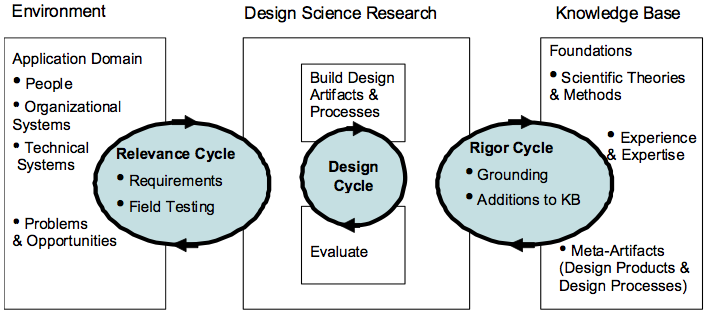
\includegraphics[width=1
	\textwidth]{design_cycles} \caption{The design cycles, figure adapted from \protect\autocite{hevner2007three}} \label{fig:design-cycles} 
\end{figure}
\begin{itemize}
	\item The \emph{relevance cycle} involves designing and running field studies with exploratory or evaluation purposes. While the former type derives requirements for technology to be implemented in prototypes, the latter type cycles between defining acceptance criteria and introducing technologies into the environment for field testing, aiming at improving artefacts until research goals are met. 
	\item The \emph{rigor cycle} includes both a continuous process of keeping design work informed by relevant grounding theories, and a retrospective effort in validation and extension of those theories. This cycle qualify the research to maintain an innovation approach able to bring research contributions. 
	\item The \emph{design cycle} rapidly iterates between the production of a prototype and its formative evaluation to gather feedbacks and refine the design. This stage is fed with requirements from the relevance cycle and theories from the rigor cycle; it returns artefacts for field test to the former and theoretical knowledge to the latter. 
\end{itemize}

To implement the main research strategy, several methods have been adopted. I used a mix of qualitative research methods to account for the unpredictability in an in-situ study \autocite{Rogers:2007gv}. Observations, interviews and researchers' notes were the primary means to collect data on the field. Scenarios and personas drove the design phase. Open source hardware and software toolkits were largely adopted to turn mockups into working prototypes. Finally questionnaires and interviews were used during prototypes formative evaluations and field tests.

The choice of these methods required the researchers to have large access to people, knowledge and protocols of organisations working in the crisis domain. This research strategy was facilitated by having crisis training organisations member of the MIRROR consortium. Moreover, throughout the duration of the work, discussions with members of the consortium and co-authored publications helped in shaping research strategies and partially influenced the work.

\section{Research activities}\label{research-activities}

This section details on activities performed and how methods have been instantiated. A chronological account of the research process is provided in Figure \ref{fig:research-activities}.
\begin{figure}
	[p] \centering 
	\includegraphics[width=1
	\textwidth]{timeline} \caption{Timeline of research activities} \label{fig:research-activities} 
\end{figure}

During the progress of the research, several activities concurrently unfolded intra and inter the \emph{relevance}, \emph{design} and \emph{rigor} cycles.

The work kicked off with two exploratory field studies aimed at understanding the crisis training domain, its needs and challenges. Soon enough early design ideas were turned into low-to-high fidelity prototypes in short iterations. 

In the central course of research, activities iterated between new prototype releases and consequent formative evaluations; often recurring to new field studies to keep the design process updated with new requirements. Prototypes presented in focus groups with workers facilitated discussions, triggering a better understanding of the domain, which in turn led to new ideas. Furthermore, prototypes facilitated the reminiscence of work experiences, brining new perspectives into the study.

In the final iterations of the work, working prototypes acted as means to validate and extend theories as part of the rigor cycle. Results from evaluations provided insights to validate and extend theories of reflective learning (rigor cycle), as reported in P6. 

Research outcomes were reported in academic publications (Chapter \ref{results}) and research contributions (Chapter \ref{contributions}) emerged. Finally the work focused on generalisation during research abroad (Appendix \ref{abroad}) and commercial exploitation of research contributions (Section \ref{exploitation-of-research-contributions}).

Throughout the process literature in reflective learning (Chapter \ref{csrl}) and sensing based interaction (Chapter \ref{interaction}) informed the design work. While the former identified \emph{what} activities and processes to trigger reflection can be enhanced with technology; the latter provided guidelines on \emph{how} to design technology artefacts.

In the following sections, a description of field studies performed, and methods adopted is provided in Section \ref{field-studies}. The production and formative evaluation of prototypes is covered by Section \ref{prototypes}.

\section{Field studies}\label{field-studies}

The primary investigation method selected to understand the crisis domain and to evaluate artefacts produced by the design cycle has been \emph{field studies}. In this work, field studies had a twofold objective. Some studies acted as exploratory research to inform the design of technology, some others as field evaluation for the tools developed; some else covered both aims.

An overview of the field studies performed between years 2011-2014, in relation with research questions and papers, is presented in Table \ref{field-studies}

\begin{table}
	[h] \centering \caption{Description of field studies performed} \label{field-studies} 
	\begin{tabular}
		{@{}lllllllll@{}} 		%\begin{tabular}{@{}p{0.3cm}p{3cm}p{0.3cm}p{0.3cm}p{3cm}p{0.25cm}p{0.25cm}p{0.25cm}p{1.5cm}}
		\toprule & & \multicolumn{2}{c}{Aim} & & \multicolumn{3}{c}{Methods} & \\
		\cline{3-4} \cline{6-8} \noalign{\smallskip} ID & \specialcell[b]{Date,\\duration} & 
		\begin{turn}
			{90}Exploratory
		\end{turn}
		& 
		\begin{turn}
			{90}Evaluation
		\end{turn}
		& Participants & 
		\begin{turn}
			{90}Observations
		\end{turn}
		& 
		\begin{turn}
			{90}Interviews
		\end{turn}
		& 
		\begin{turn}
			{90}Questionnaires
		\end{turn}
		& Papers \\
		\midrule \noalign{\smallskip} F1 & \specialcell[t]{Mar. 2011,\\2 days} & \textbullet & & several teams & \textbullet & \textbullet & & P1 \\
		F2 & \specialcell[t]{Oct. 2011,\\3 days} & \textbullet & & \specialcell[t]{several teams,\\1 manager} & \textbullet & \textbullet & & P1, P3 \\
		F3 & \specialcell[t]{Oct. 2012,\\2 days} & \textbullet & \textbullet & \specialcell[t]{5 field workers,\\1 manager} & \textbullet & \textbullet & & P1, P3 \\
		F4 & \specialcell[t]{Apr. 2013,\\3 days} & \textbullet & \textbullet & \specialcell[t]{4 field workers,\\1 manager} & \textbullet & \textbullet & \textbullet & P1, P3, P2 \\
		F5* & \specialcell[t]{Dec. 2013,\\30 days} & & \textbullet & 8 field workers & & & \textbullet & P2, P3, P6 \\
		F6 & \specialcell[t]{Apr. 2014,\\2 days} & & \textbullet & \specialcell[t]{27 field workers,\\1 manager} & \textbullet & & \textbullet & P2, P3, P6 \\
		\noalign{\smallskip} \hline \noalign{\smallskip} \multicolumn{9}{l}{*The author was not present during the study} \\
		\bottomrule 
	\end{tabular}
\end{table}

The setting for the majority of the studies was medium to large scale physical simulation of crisis work (drills). A description of a typical physical simulation was provided in Chapter \ref{crisis}. Only the first exploratory study (F1 in Table \ref{field-studies}) took place during attendance to a real crisis management event. Objectives of those simulations were to train workers against protocols, rescue procedures, and test of equipments. Notably, the observed events also offered opportunities for team building and sharing of experiences, as part of official an unofficial social gatherings.

The observed training events, involved personnel from a range of crisis management organisations operating in northern Italy, coordinated by \emph{ANPAS-Piemonte}\footnote{ANPAS-Piemonte crisis management organisation - http://anpas.piemonte.it} and \emph{SEIRS}\footnote{SEIRS crisis management organisation - http://seirs.org} organisations. Those institutions were selected because of being affiliated to the MIRROR consortium, which facilitated access to resources and personal. A wide range of roles were observed, including field workers (firefighters, paramedics, police agents), team coordinators, disaster manager, technical and radio staff. The number of participants to our studies varied between dozens of workers observed in the exploratory studies to smaller groups who where actively involved during interviews and prototypes evaluations.

Observations, researcher notes and interviews were the primary means to collect data. In addition questionnaires were employed during evaluation studies.

Workers were shadowed while performing rescue work. To this respect, my role as observer strived to be, as defined by Walsham \autocite*{Walsham:2006bo}, \emph{neutral}; meaning that people being shadowed shouldn't perceive the researcher as biased by previous views on people, processes or organisations. Video recording, performed with both handheld and head-mounted cameras worn by simulations' participants, provided multiple point of views on the observed events. Qualitative data collection methods were supplemented by descriptions of protocols, procedures and best practices provided by the organisations involved in the studies. Data captured were handled in observance of NTNU and MIRROR policies. No compensation was given to the workers upon participation to the studies.

Data collected from researchers' notes, interviews and questionnaires, together with video recording and logs were analysed with qualitative research methods \autocite{robson1993real}. The focus of the analysis was twofold.

During exploratory studies the focus of attention was on how practitioners capture aspects of their work experiences. It allowed to identify on one end what information is relevant for reflection; on the other end what technology to capture information is already in use or is desired. The outcome of this phase produced a set of requirements to drive the design of technology; including challenges, system requirements, scenarios and personas. This result feeds the \emph{design cycles}, for the construction of prototypes.

During evaluation studies the focus was on measuring how well prototypes perform against user acceptance, usability of the systems, and impact on learning. Selected workers were provided with prototypes for test during field work. Workers were walked thru the use of technology by a researcher and a set of tasks to be accomplished was given to each participant. Tasks had to be performed during crisis work, to assess the compatibility for the technology and user interfaces with rescue protocols. Participants' interactions with the technology was observed and video recorded with wearable cameras; in addition prototypes were configured to log modes of operation.

After each test, researchers followed up with observations, interviews and questionnaires. Questionnaires offered a high-level quantification of feedback, while observations and interviews aimed to ground this feedback in the context of usage. Questionnaires in use during the evaluations were adapted from the MIRROR evaluation toolbox \autocite{Knipfer:2012vi}, which provides surveys to measure user acceptance, perceived learning success, and the intention to change behaviour. These questionnaires are a generic instrument that build on the Kirkpatrick framework \autocite{kirkpatrick2009evaluating} \todo{worth mentioning it or could I get questions about the framwork?} and have been developed through an extensive survey of literature on reflective learning and in cooperation with participants from different workplace settings.

Gather access to people for the studies has proven to be challenging. Training exercises aimed at re-creating aspects of stress and unpredictability typical of real emergencies, for this reason workers were not always prone to share information with researchers. Even more, sometimes the presence of researchers has been seen as disruptive for the training activities. The time of the events set apart for debriefing and collaborative reflection was also very limited. Despite those challenges I was able to gather enough information to drive  design work. This is mostly thanks to the number of studies performed and to the relationship maintained throughout the years with a group of five workers who I deeply thank.\todo{should I move this paragraph to the evaluation chapter?}

\section{Design iterations}\label{design-iterations}

A large amount of time was dedicated to the design and construction of technology artefacts. The prototyping work was driven by requirements, scenarios and personas generated during field studies. The design process followed a \emph{user centred approach} \autocites{MAGUIRE:2001dp}{Gulliksen:2003hd}.

A total of eight prototypes were produced, including apps, wearable sensors and technology-augmented board games. Table \ref{prototypes} overviews the prototypes developed, tools and technologies used during development, relation with the papers and field studies.
\begin{table}
	[!p] \centering \caption{List of prototypes built} \label{prototypes} 
	\begin{threeparttable}
		\begin{tabular}
			{@{}lllllllll@{}} \toprule & & & & \multicolumn{3}{c}{Development} & & \\
			\cline{5-7} \noalign{\smallskip} \specialcell[b]{ID\\Ver.} & Name & Released & Prototyping tools & 
			\begin{turn}
				{90}Software
			\end{turn}
			& 
			\begin{turn}
				{90}Hardware
			\end{turn}
			& 
			\begin{turn}
				{90}Casing
			\end{turn}
			& Papers & \specialcell[b]{Field\\studies} \\
			\midrule \noalign{\smallskip} C1 & CroMAR & Jul. 2011 & iOS, & \textbullet & & & P1,P2 & F1,F2 \\
			C2 & & Jul. 2012 & Augmented Reality & \textbullet & & & P2 & F3, F4 \\
			\hline \noalign{\smallskip} W1 & WATCHiT & Jan. 2012 & Arduino, Textiles & \textbullet & \textbullet & & P3 & F2 \\
			W2 & & Aug. 2012 & ZigBee, Bluetooth & \textbullet & \textbullet & & P3 & F2 \\
			W3 & & Sept. 2012 & & \textbullet & \textbullet & & P3 & F3, F4 \\
			W4 & & Aug. 2013 & & \textbullet & \textbullet & \textbullet & P2, P3 & F5, F6 \\
			\hline \noalign{\smallskip} D1 & Don't Panic & Mar. 2013 & Paper, wood & & & \textbullet & P4, P5 & F1 \\
			D2 & & Aug. 2013 & \specialcell[t]{Sifteo, RapsberryPi\\Laser cut} & \textbullet & \textbullet & \textbullet & P5 & F1 \\
			\bottomrule 
		\end{tabular}
		\begin{tablenotes}
			\item 
			\includegraphics[width=\linewidth]{prototypes} 
		\end{tablenotes}
	\end{threeparttable}
\end{table}

Building each prototype involved a mix of software, hardware and construction development. Software was written for a variety of systems in different languages. The development of hardware included design, production and test of electronic circuits. In some prototypes the circuits developed were embedded in cases that were custom-designed and produced in plastic or wood. The design of the appearance for the resulting software/hardware hybrid artefact aimed either at protecting electronic circuits during field test or to provide specific affordances for interaction.

During development I largely adopted rapid prototyping techniques in order to keep design iterations shorts and produce incremental improvements based on frequent feedbacks exchange with end users. To this end a wide range of open source toolkit were used, including Arduino\footnote{Arduino platform - http://arduino.cc} and RaspberryPi\footnote{RaspberryPi platform - http://raspberrypi.org} hardware development platforms. Digital manufacturing techniques were largely adopted, including CAD softwares, 3D printing and laser-cut production. These activities were essential to the development of knowledge to the investigation of RQ3. Building prototypes I was often helped by a few students who have written master theses related to the topics presented in this thesis.\todo{leave?}

After each prototype was built, a formative evaluation followed. Frequent user testing allowed for maintaining a user-centred design perspective, to introduce new ideas into the process, and to test prototypes in a controlled setting before releasing them for field testing.
\begin{table}
	[h] \centering \caption{Description of focus groups performed} \label{labtests} 
	\begin{tabular}
		{@{}lllllllll@{}} \toprule ID & Date & Participants & Prototypes tested \\
		\midrule G1 & Apr. 2012 & 9 filed workers & W1, D1 \\
		G2 & May 2012 & 1 disaster manager & C1, W1 \\
		G3 & Jul. 2013 & 3 field workers, 1 manager & D2 \\
		G4 & Sept. 2013 & 8 IT students, 4 HCI experts & D2 \\
		\bottomrule 
	\end{tabular}
\end{table}

To this intent, focus groups with crisis workers were performed. A list of focus groups performed, and prototypes tested is depicted in Table \ref{labtests}. Focus groups with workers were essential for fuelling the design activity. Moreover, meetings often saw the participation of the same workers who were perviously shadowed during physical simulations. It was therefore possible to ground discussions into specific episodes previously observed on the field.

\begin{figure}
	[tbh] \centering 
	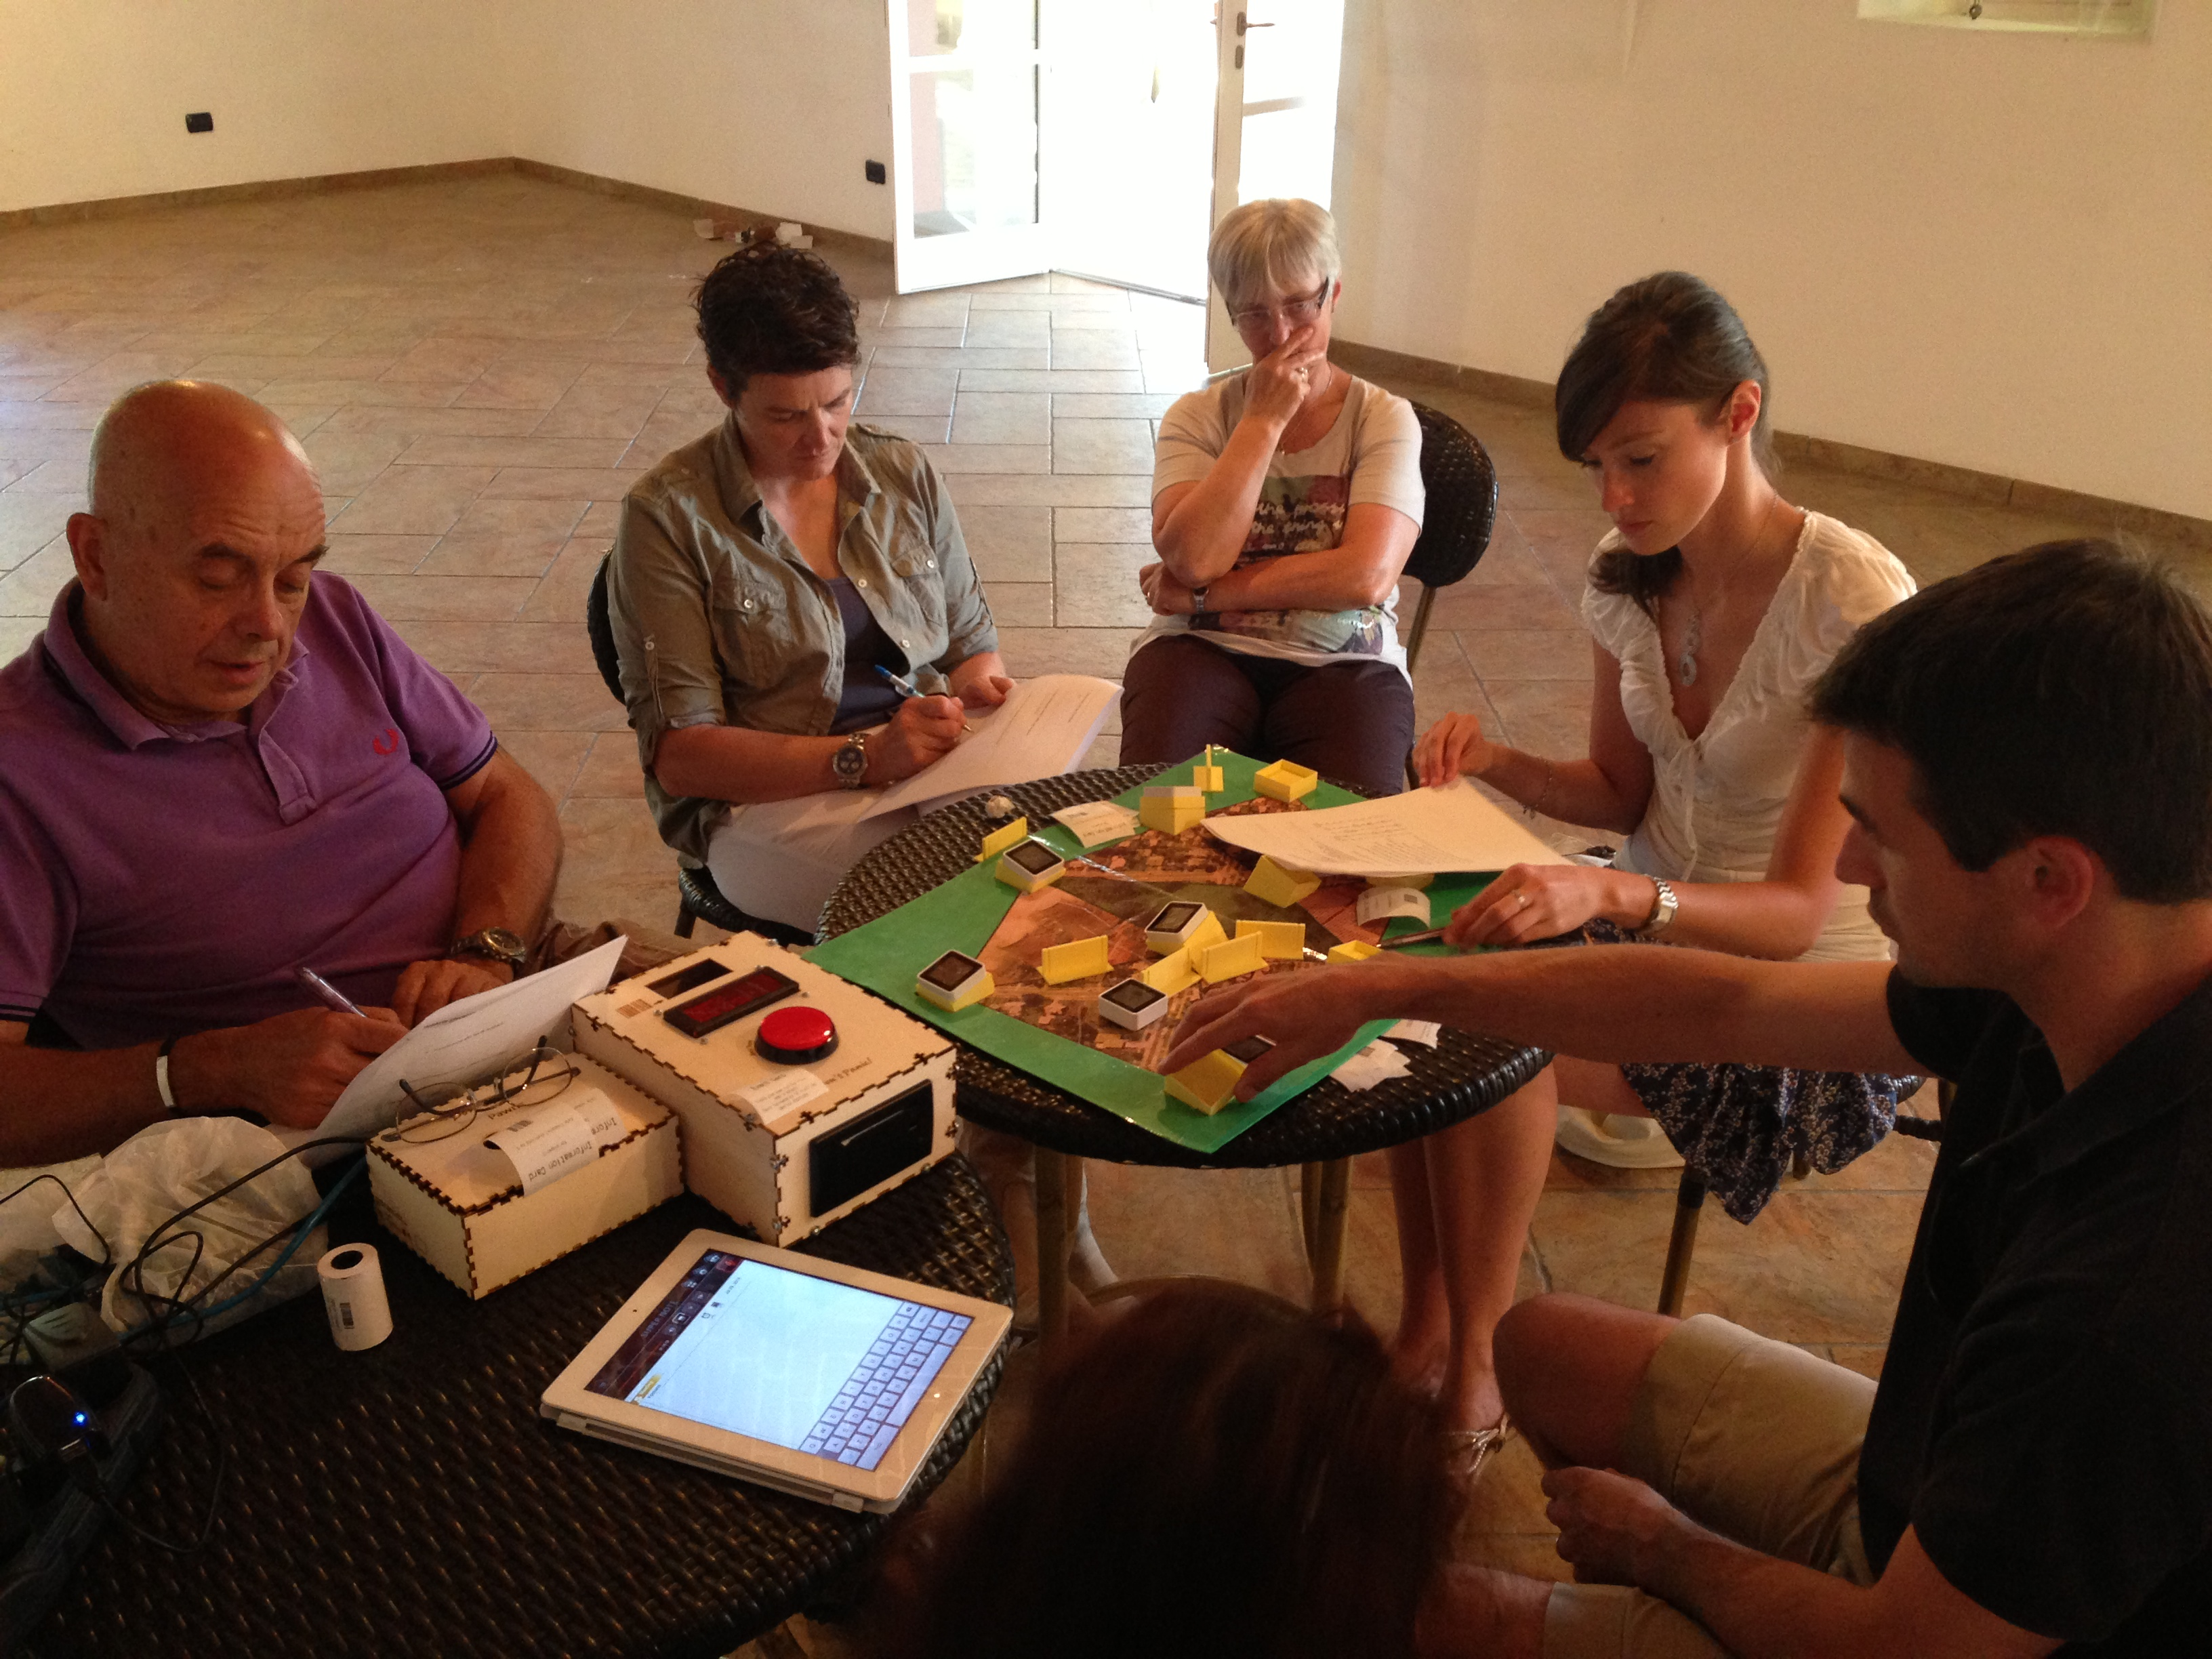
\includegraphics[width=1
	\textwidth]{d2_prototype} \caption{Participants of the G3 group filling in SUS questionnaires, after the test of D2 prototype} \label{fig:focus-group} 
\end{figure}

During focus groups low and high fidelity prototypes were evaluated. The typical setting of focus groups performed is represented in Figure \ref{fig:focus-group}. Low-fidelity prototypes acted as technology probes \autocite{Hutchinson:2003il}. Despite their evident usability issues, they were essential to create new scenarios of use and identify technological and usage challenges. Higher-fidelity prototypes underwent usability tests \autocite{Dumas:2009th} using System Usability Scale (SUS) \autocite[ pag.189]{jordan1996usability}.

In the following chapters the papers that added up to the results of this thesis are presented.